\section{Results}
\label{sec:results}

\subsection{Pareto Characterization of LLM Kernels}
To evaluate the existence and shape of the latency-energy Pareto frontier, we performed exhaustive grid searches over the entire configuration space for each kernel. Figure \ref{fig:rmsnorm_pareto} and Figure \ref{fig:matmul_pareto} illustrate the results for RMSNorm (Shape: $4096 \times 4096$) and Tiled GEMM (Shape: $4096^3$), respectively.

\begin{figure}[ht]
\centering
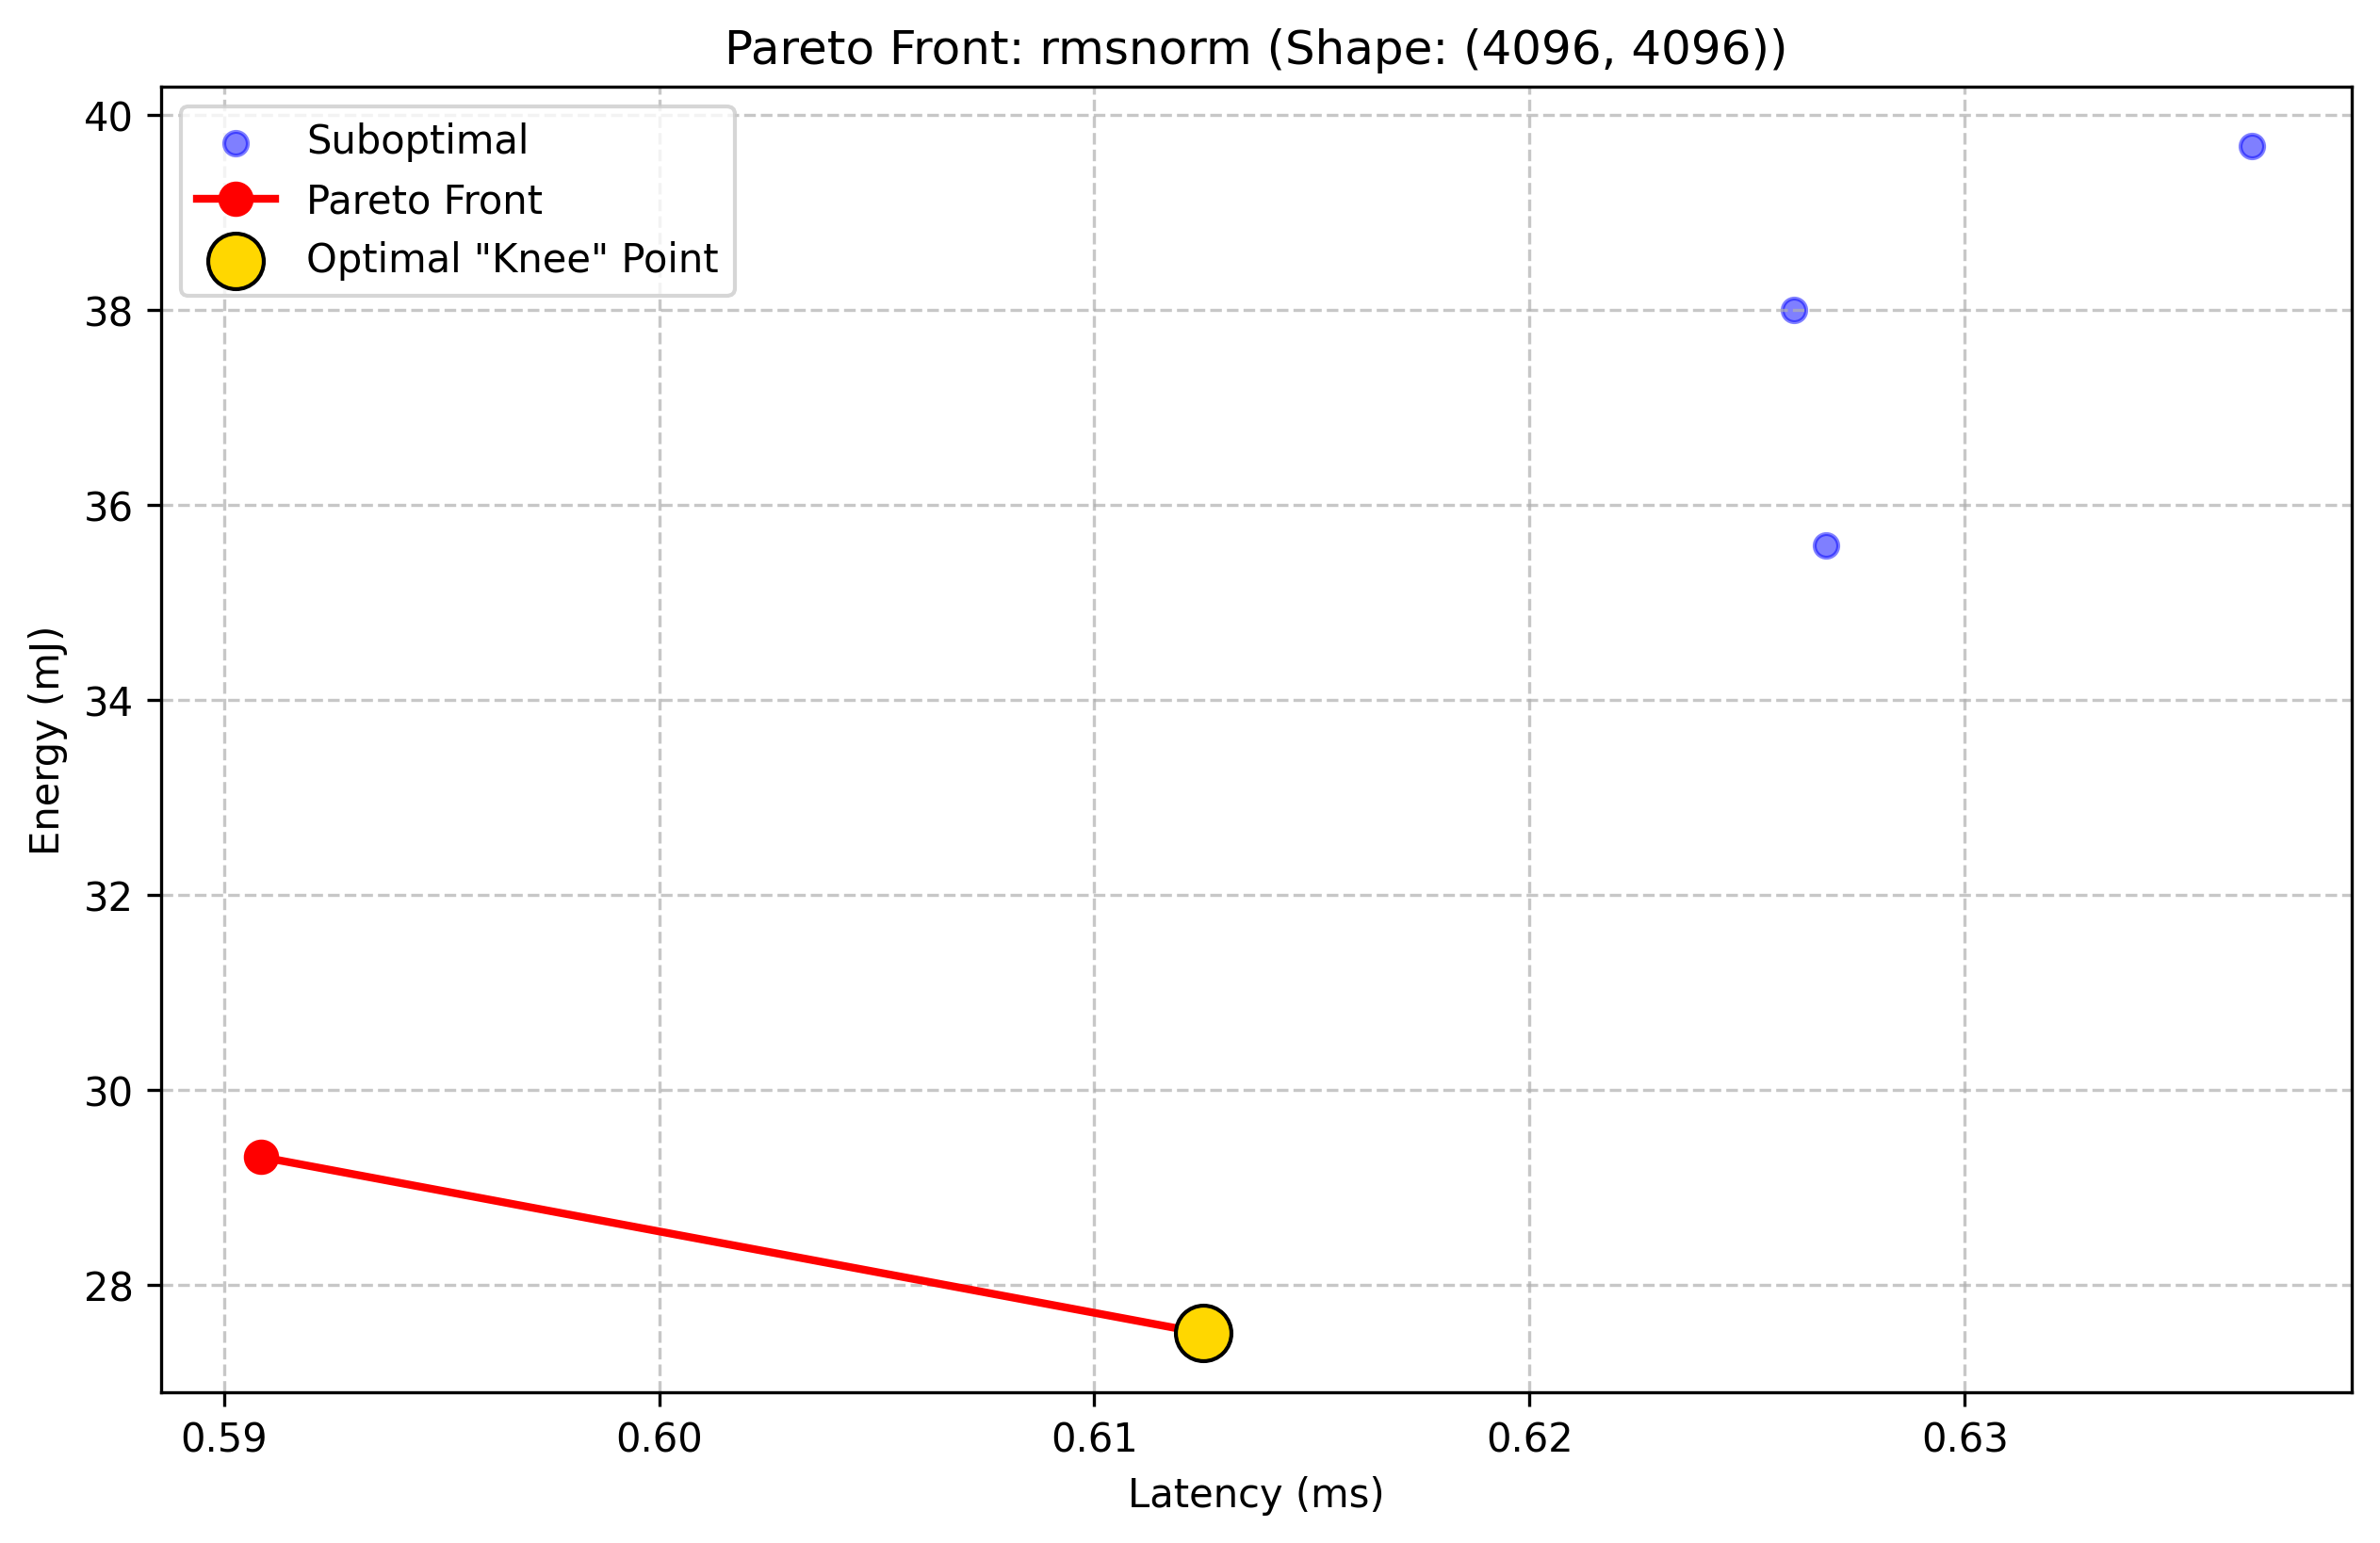
\includegraphics[width=\linewidth]{figures/rmsnorm_4096_4096_pareto.png}
\caption{Latency vs. Energy for RMSNorm ($4096 \times 4096$). The energy-optimal configuration uses 16 warps, while the latency-optimal configuration uses 32 warps.}
\label{fig:rmsnorm_pareto}
\end{figure}

\begin{figure}[ht]
\centering
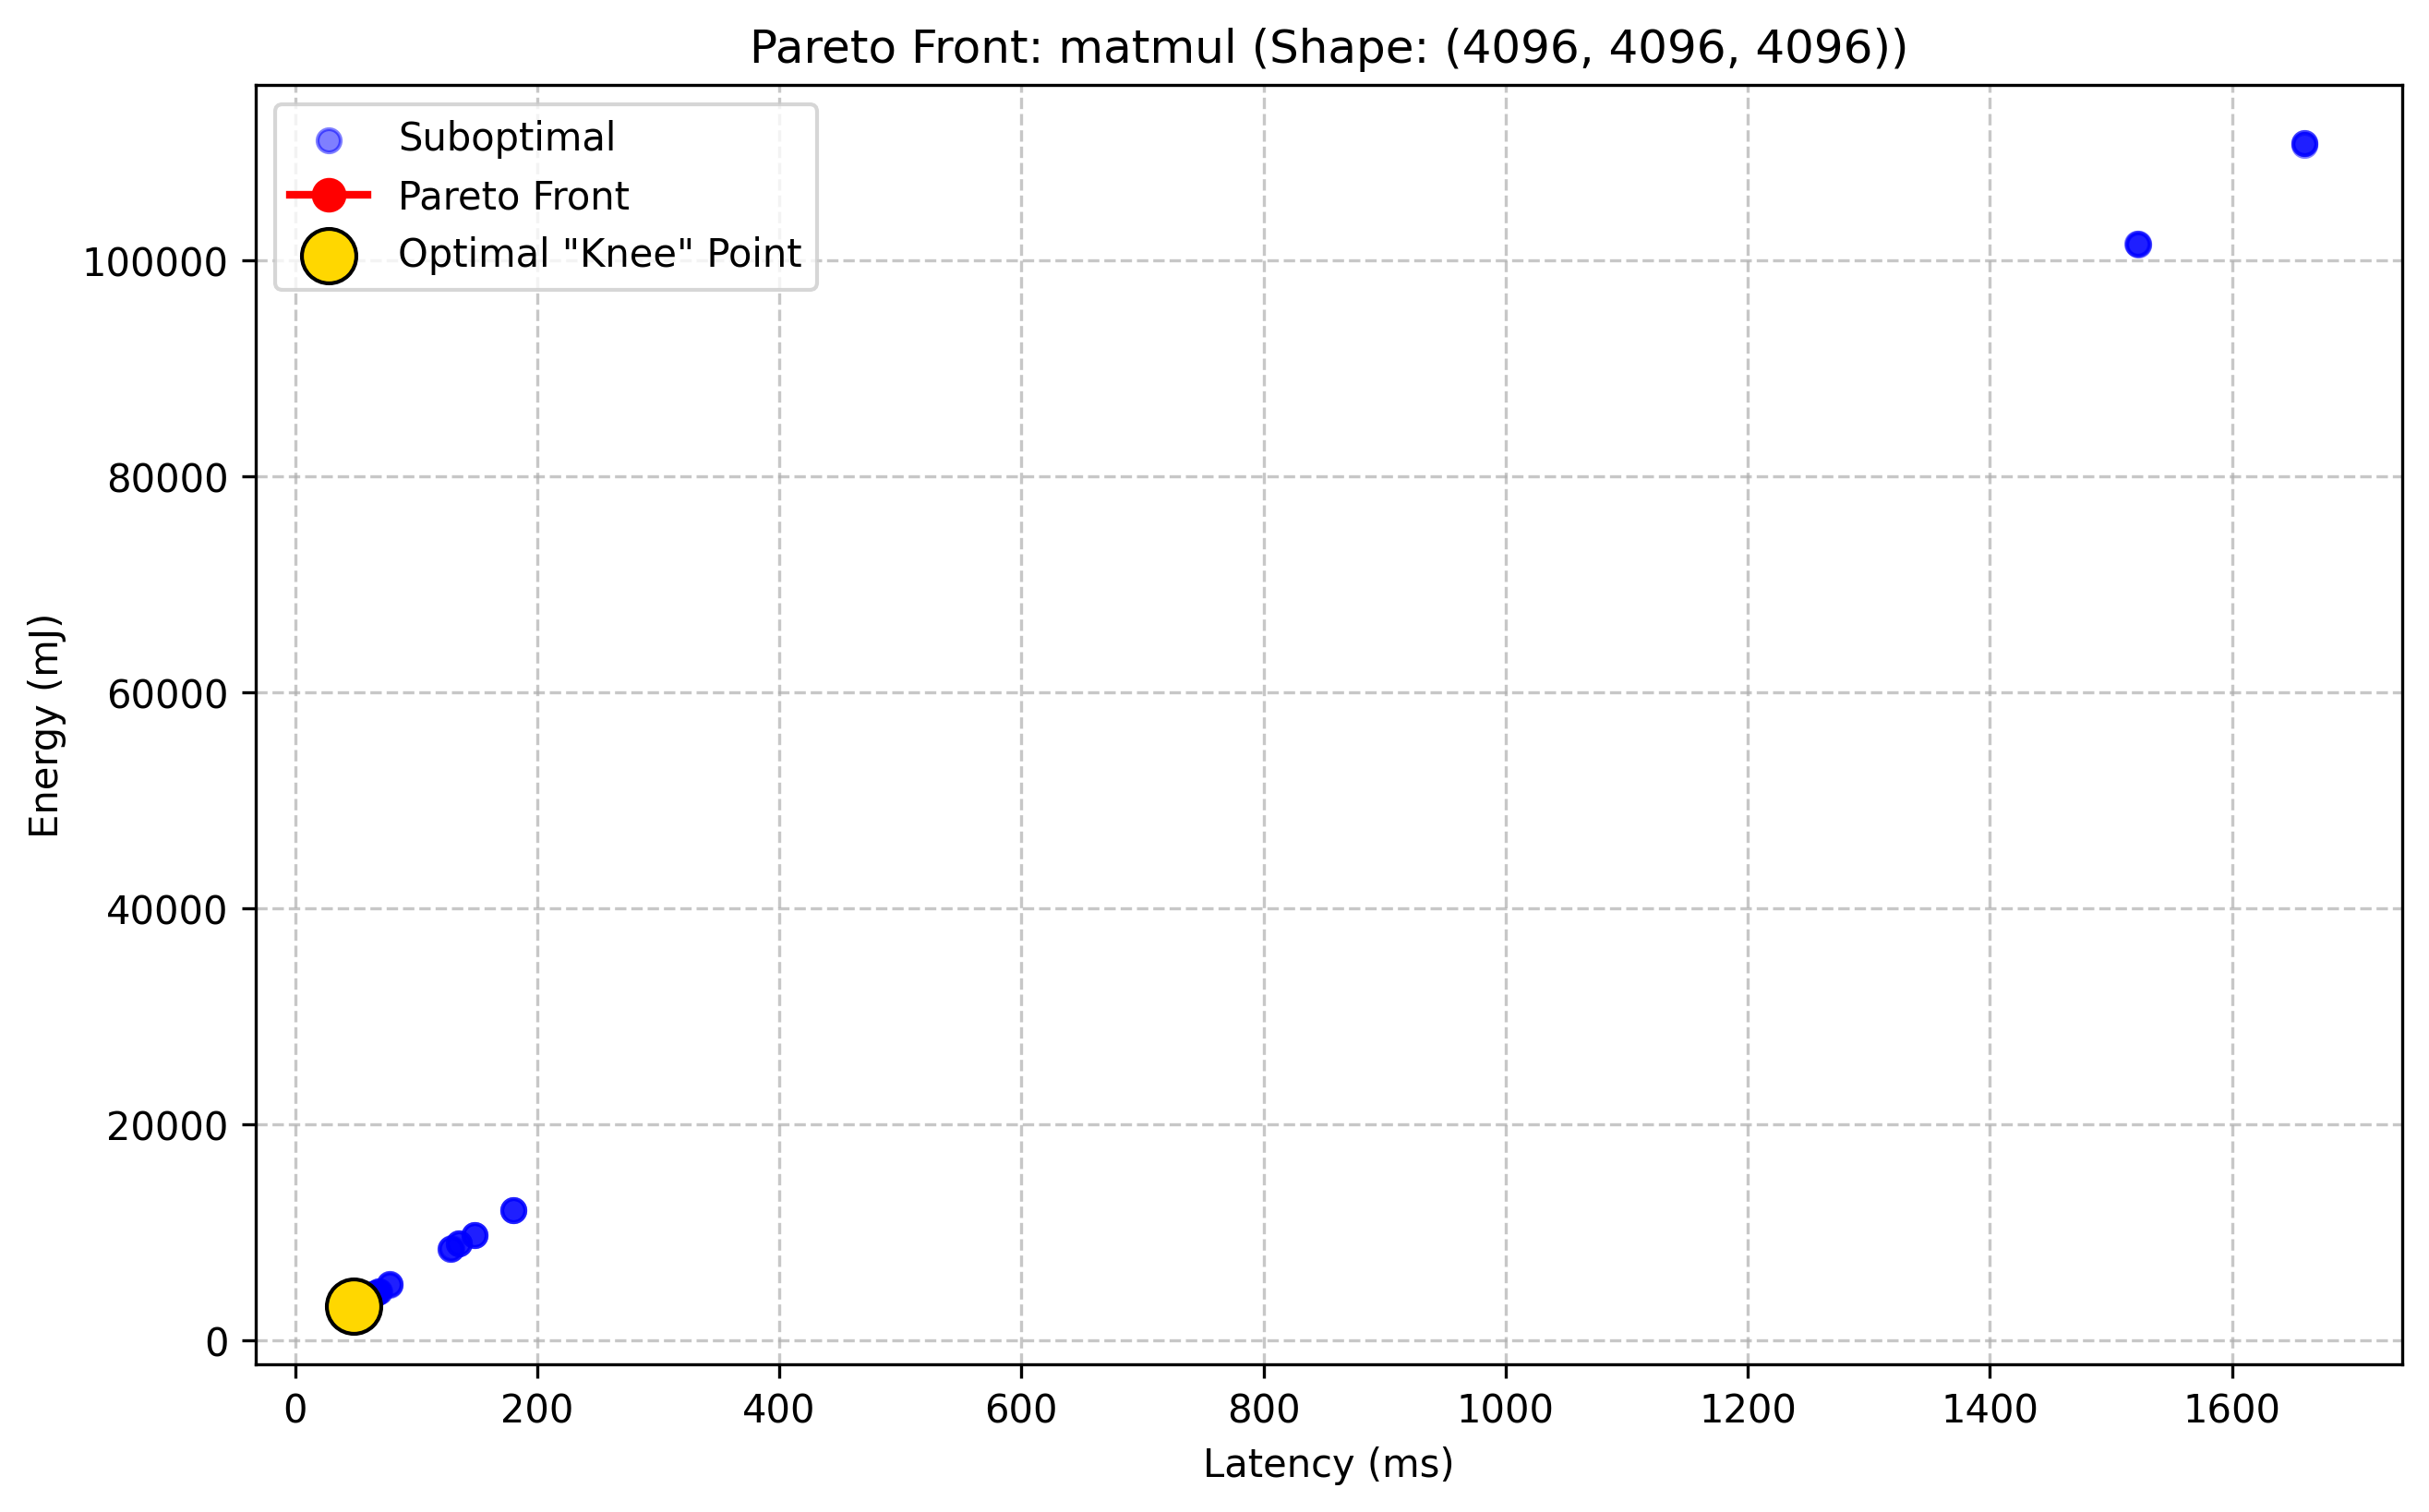
\includegraphics[width=\linewidth]{figures/matmul_4096_4096_4096_pareto.png}
\caption{Latency vs. Energy for Tiled GEMM ($4096^3$). The compute-bound nature of this kernel leads to closely overlapping optimal regions, though tradeoff knees still exist.}
\label{fig:matmul_pareto}
\end{figure}

Our empirical results confirm that for memory-bound kernels, the optimal configuration heavily depends on the target objective. For instance, in the RMSNorm benchmark (Figure \ref{fig:rmsnorm_pareto}), minimizing latency requires deploying 32 active warps to fully saturate memory bandwidth, completing execution in $0.59$ ms. However, this incurs substantial idle power dissipation. By backing off to 16 warps, we achieved the energy-optimal configuration of $27.50$ mJ, yielding significant power savings with a marginal impact on throughput.

\subsection{Heatmap Analysis of Tiled GEMM}
To better visualize the gradient of energy efficiency across hyperparameters, we plotted the search space of Tiled GEMM. Figure \ref{fig:matmul_heatmap} demonstrates the impact of varying Block Size and Warp counts. Configurations with excessively large blocks but insufficient warps to hide memory latency exhibit massive energy spikes, confirming that sub-optimal compiler decisions actively degrade power efficiency.

\begin{figure}[ht]
\centering
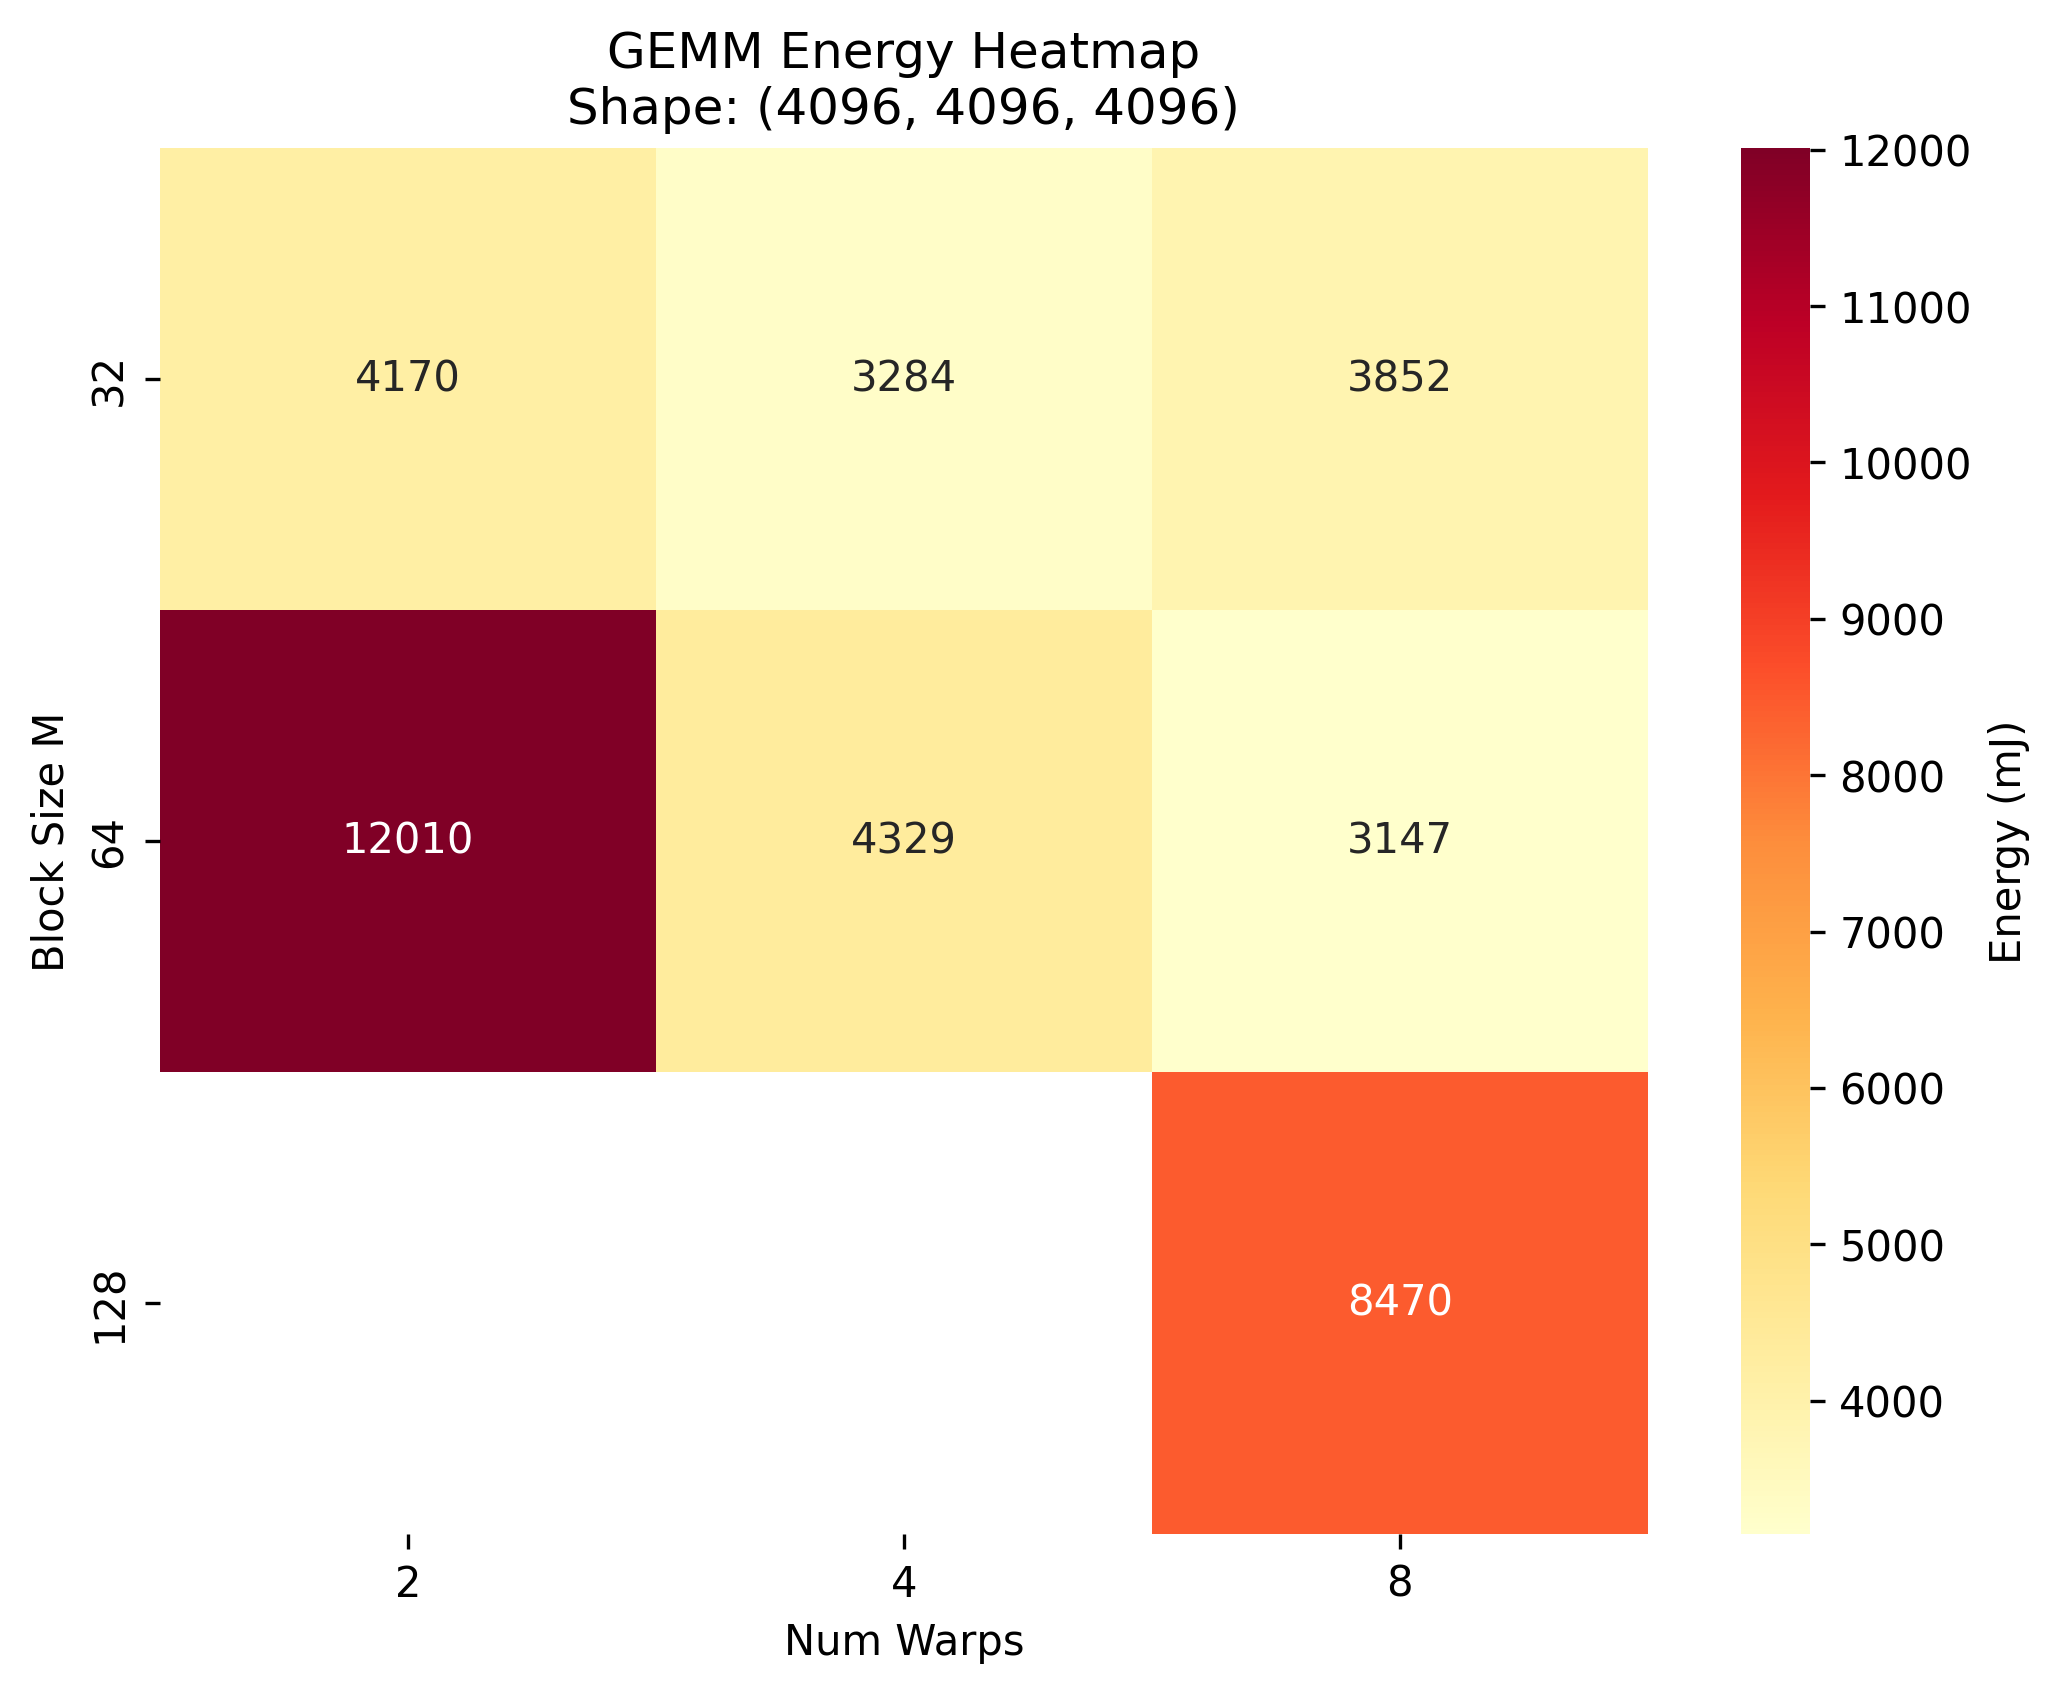
\includegraphics[width=\linewidth]{figures/matmul_4096_4096_4096_heatmap.png}
\caption{Latency vs. Energy Heatmap for Tiled GEMM ($4096^3$). Warmer colors indicate higher latency. The non-linear distribution proves that configuration selection heavily dictates energy draw.}
\label{fig:matmul_heatmap}
\end{figure}

\subsection{Mixed-Bound Kernels: Fused Causal Attention}
We also evaluated Fused Causal Attention, a heavily utilized mixed-bound kernel popularized by FlashAttention. Figure \ref{fig:attention_pareto} shows the results for a standard sequence length ($2048 \times 64$). Unlike pure memory-bound operations, Attention requires balancing shared memory capacity with high compute throughput. We found the latency-optimal configuration (completed in $7.27$ ms) used \texttt{num\_stages}: 3, whereas the energy-optimal configuration (costing $486.70$ mJ) used \texttt{num\_stages}: 4. This reinforces that deeper software pipelines often act as energy regulators.

\begin{figure}[ht]
\centering
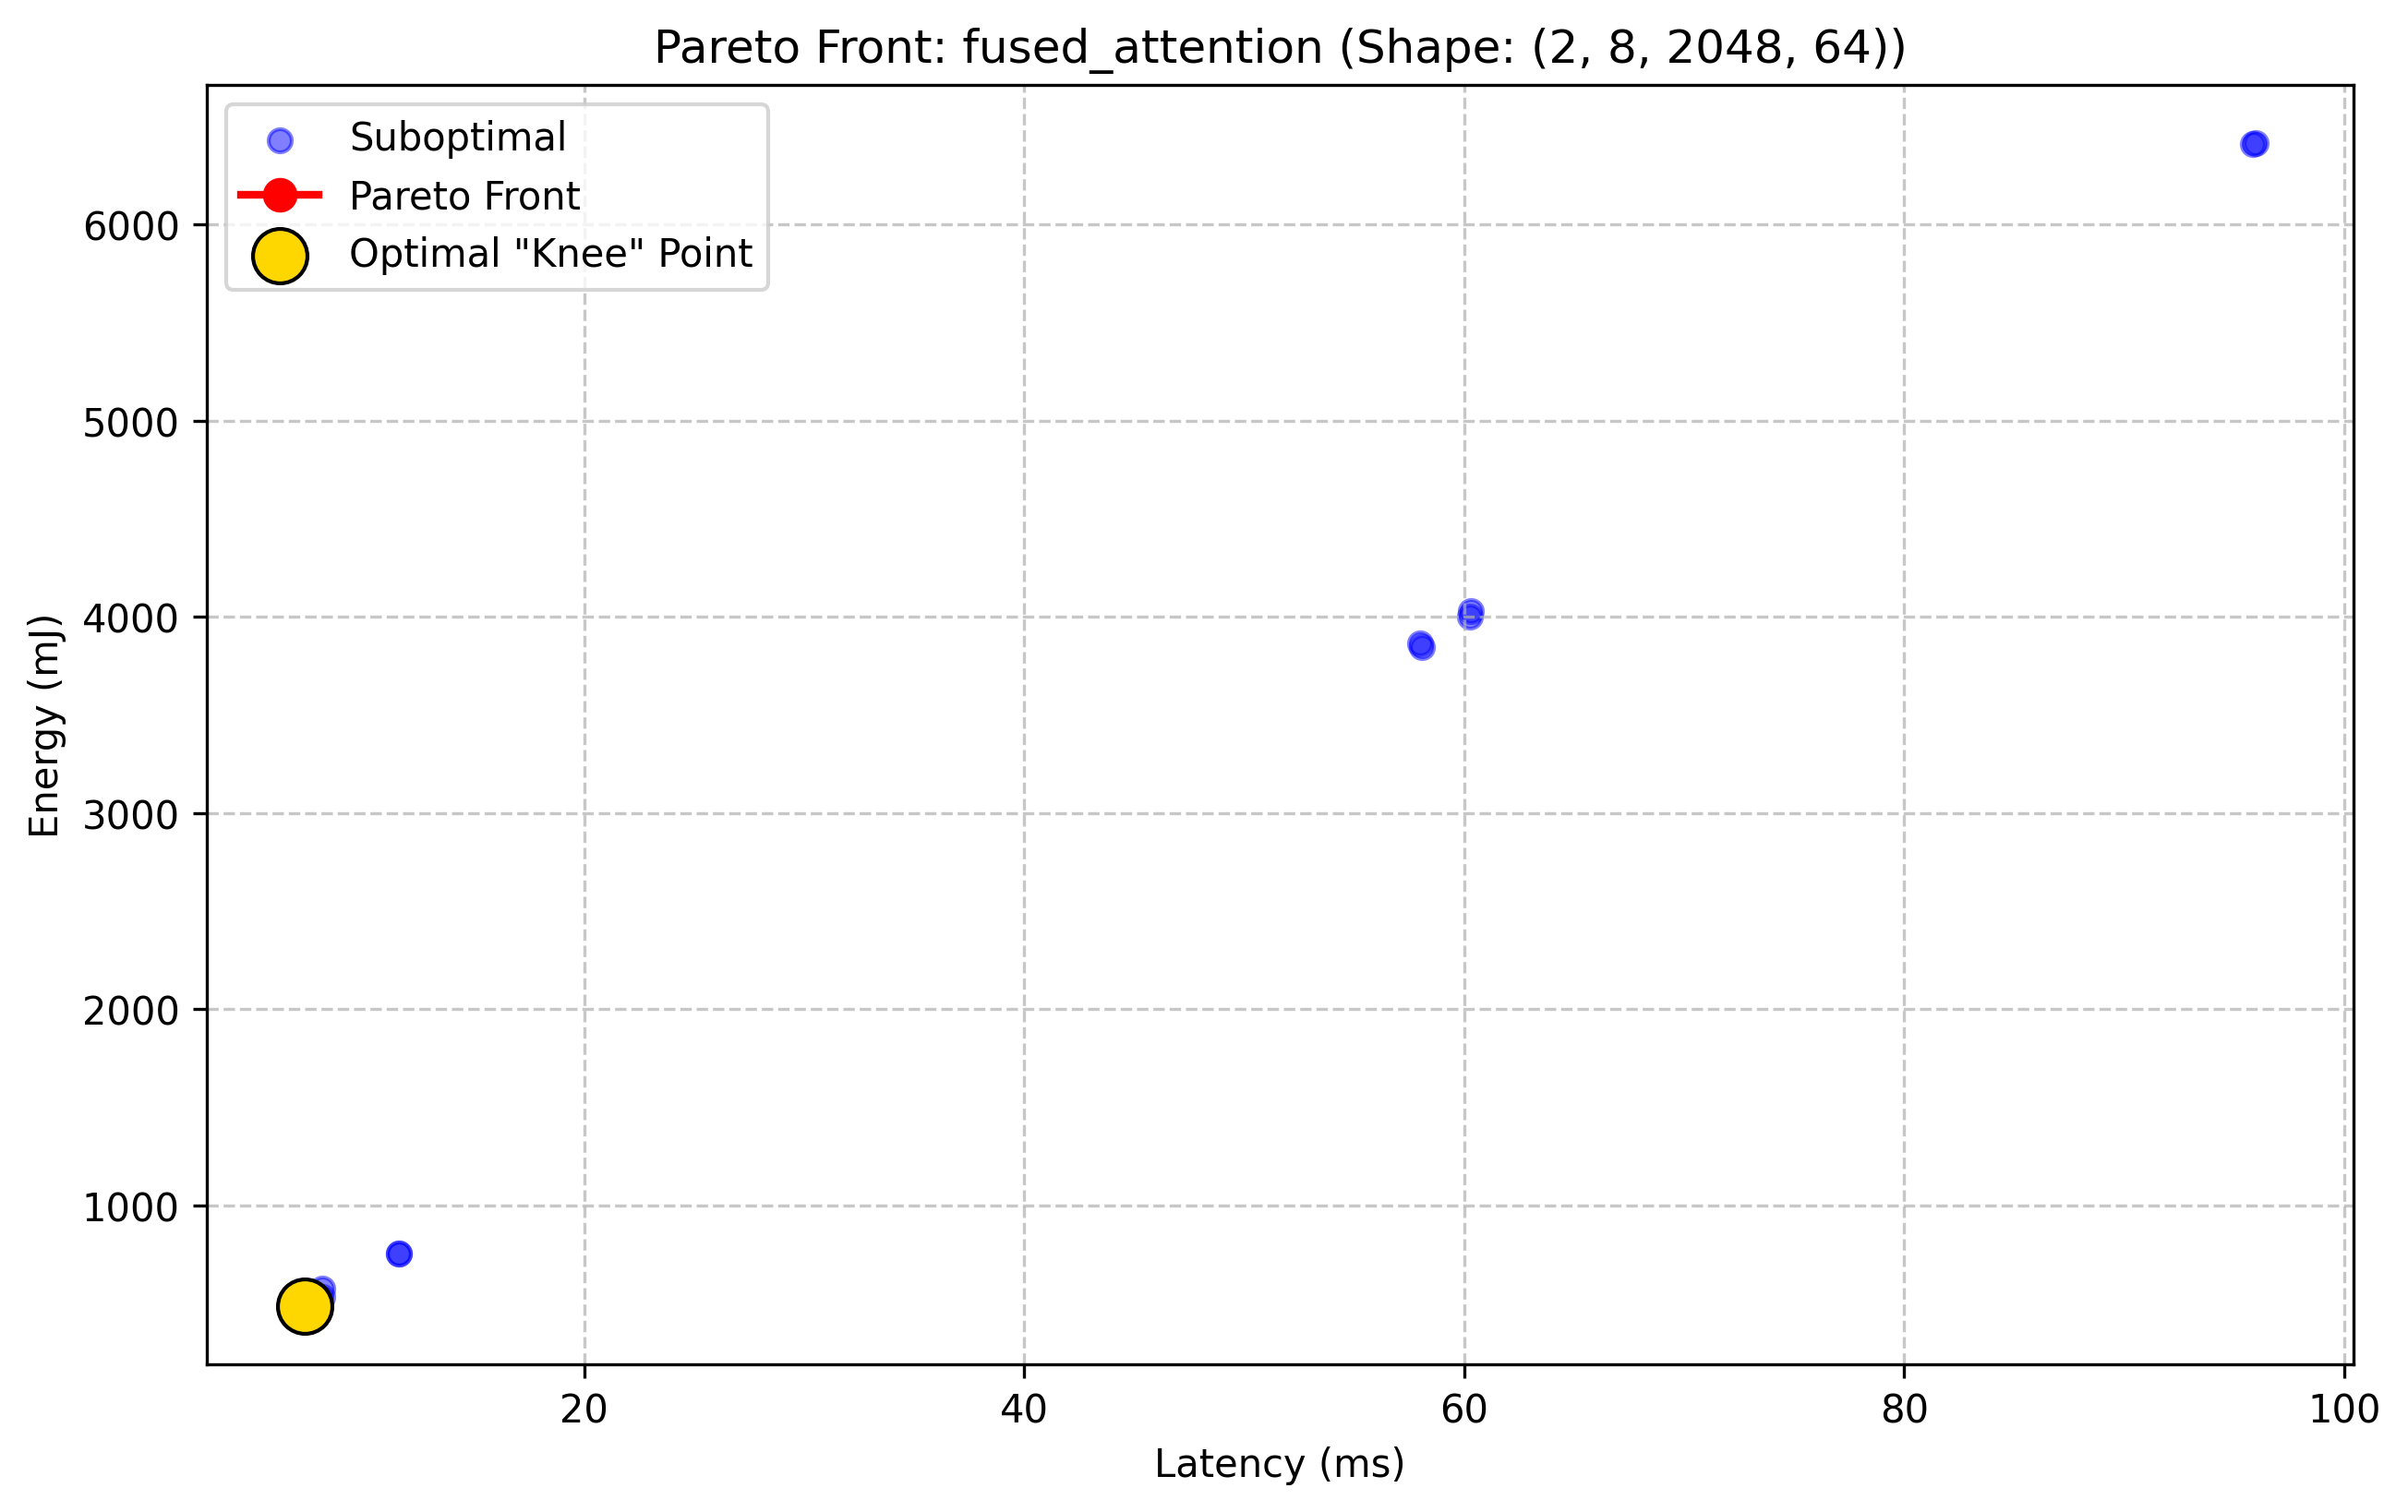
\includegraphics[width=\linewidth]{figures/fused_attention_2_8_2048_64_pareto.png}
\caption{Latency vs. Energy for Fused Causal Attention (SeqLen: 2048). Energy optimization requires deeper pipeline stages to smooth memory transitions.}
\label{fig:attention_pareto}
\end{figure}

\subsection{Configuration Shape Topology}
Our cross-shape stability analysis revealed that the energy-optimal configuration systematically differs from the latency-optimal one in specific ways:
\begin{itemize}
    \item \textbf{Under-provisioning Warps:} Across Vector Addition, Softmax, and RMSNorm, the energy optimizer consistently halves the number of active warps compared to the latency optimizer (e.g., 4 warps vs 16 warps for Vector Add).
    \item \textbf{Software Pipelining:} For compute-bound and mixed kernels, the energy optimizer favors deeper pipelining (\texttt{num\_stages}: 4) compared to the latency optimizer (\texttt{num\_stages}: 2 or 3), suggesting that smoother memory-to-register transitions draw less peak power.
\end{itemize}

\subsection{Cost-Model Guided Search}
Given the exponential size of the Tiled GEMM configuration space, exhaustive sweeping requires over 40 minutes per shape on a T4 GPU. We deployed a multi-objective Optuna TPE search with a budget of 20 trials. Figure \ref{fig:optuna_pareto} demonstrates that the machine-learning-guided search successfully approximated the true Pareto frontier discovered by the exhaustive grid in a fraction of the time.

\begin{figure}[ht]
\centering
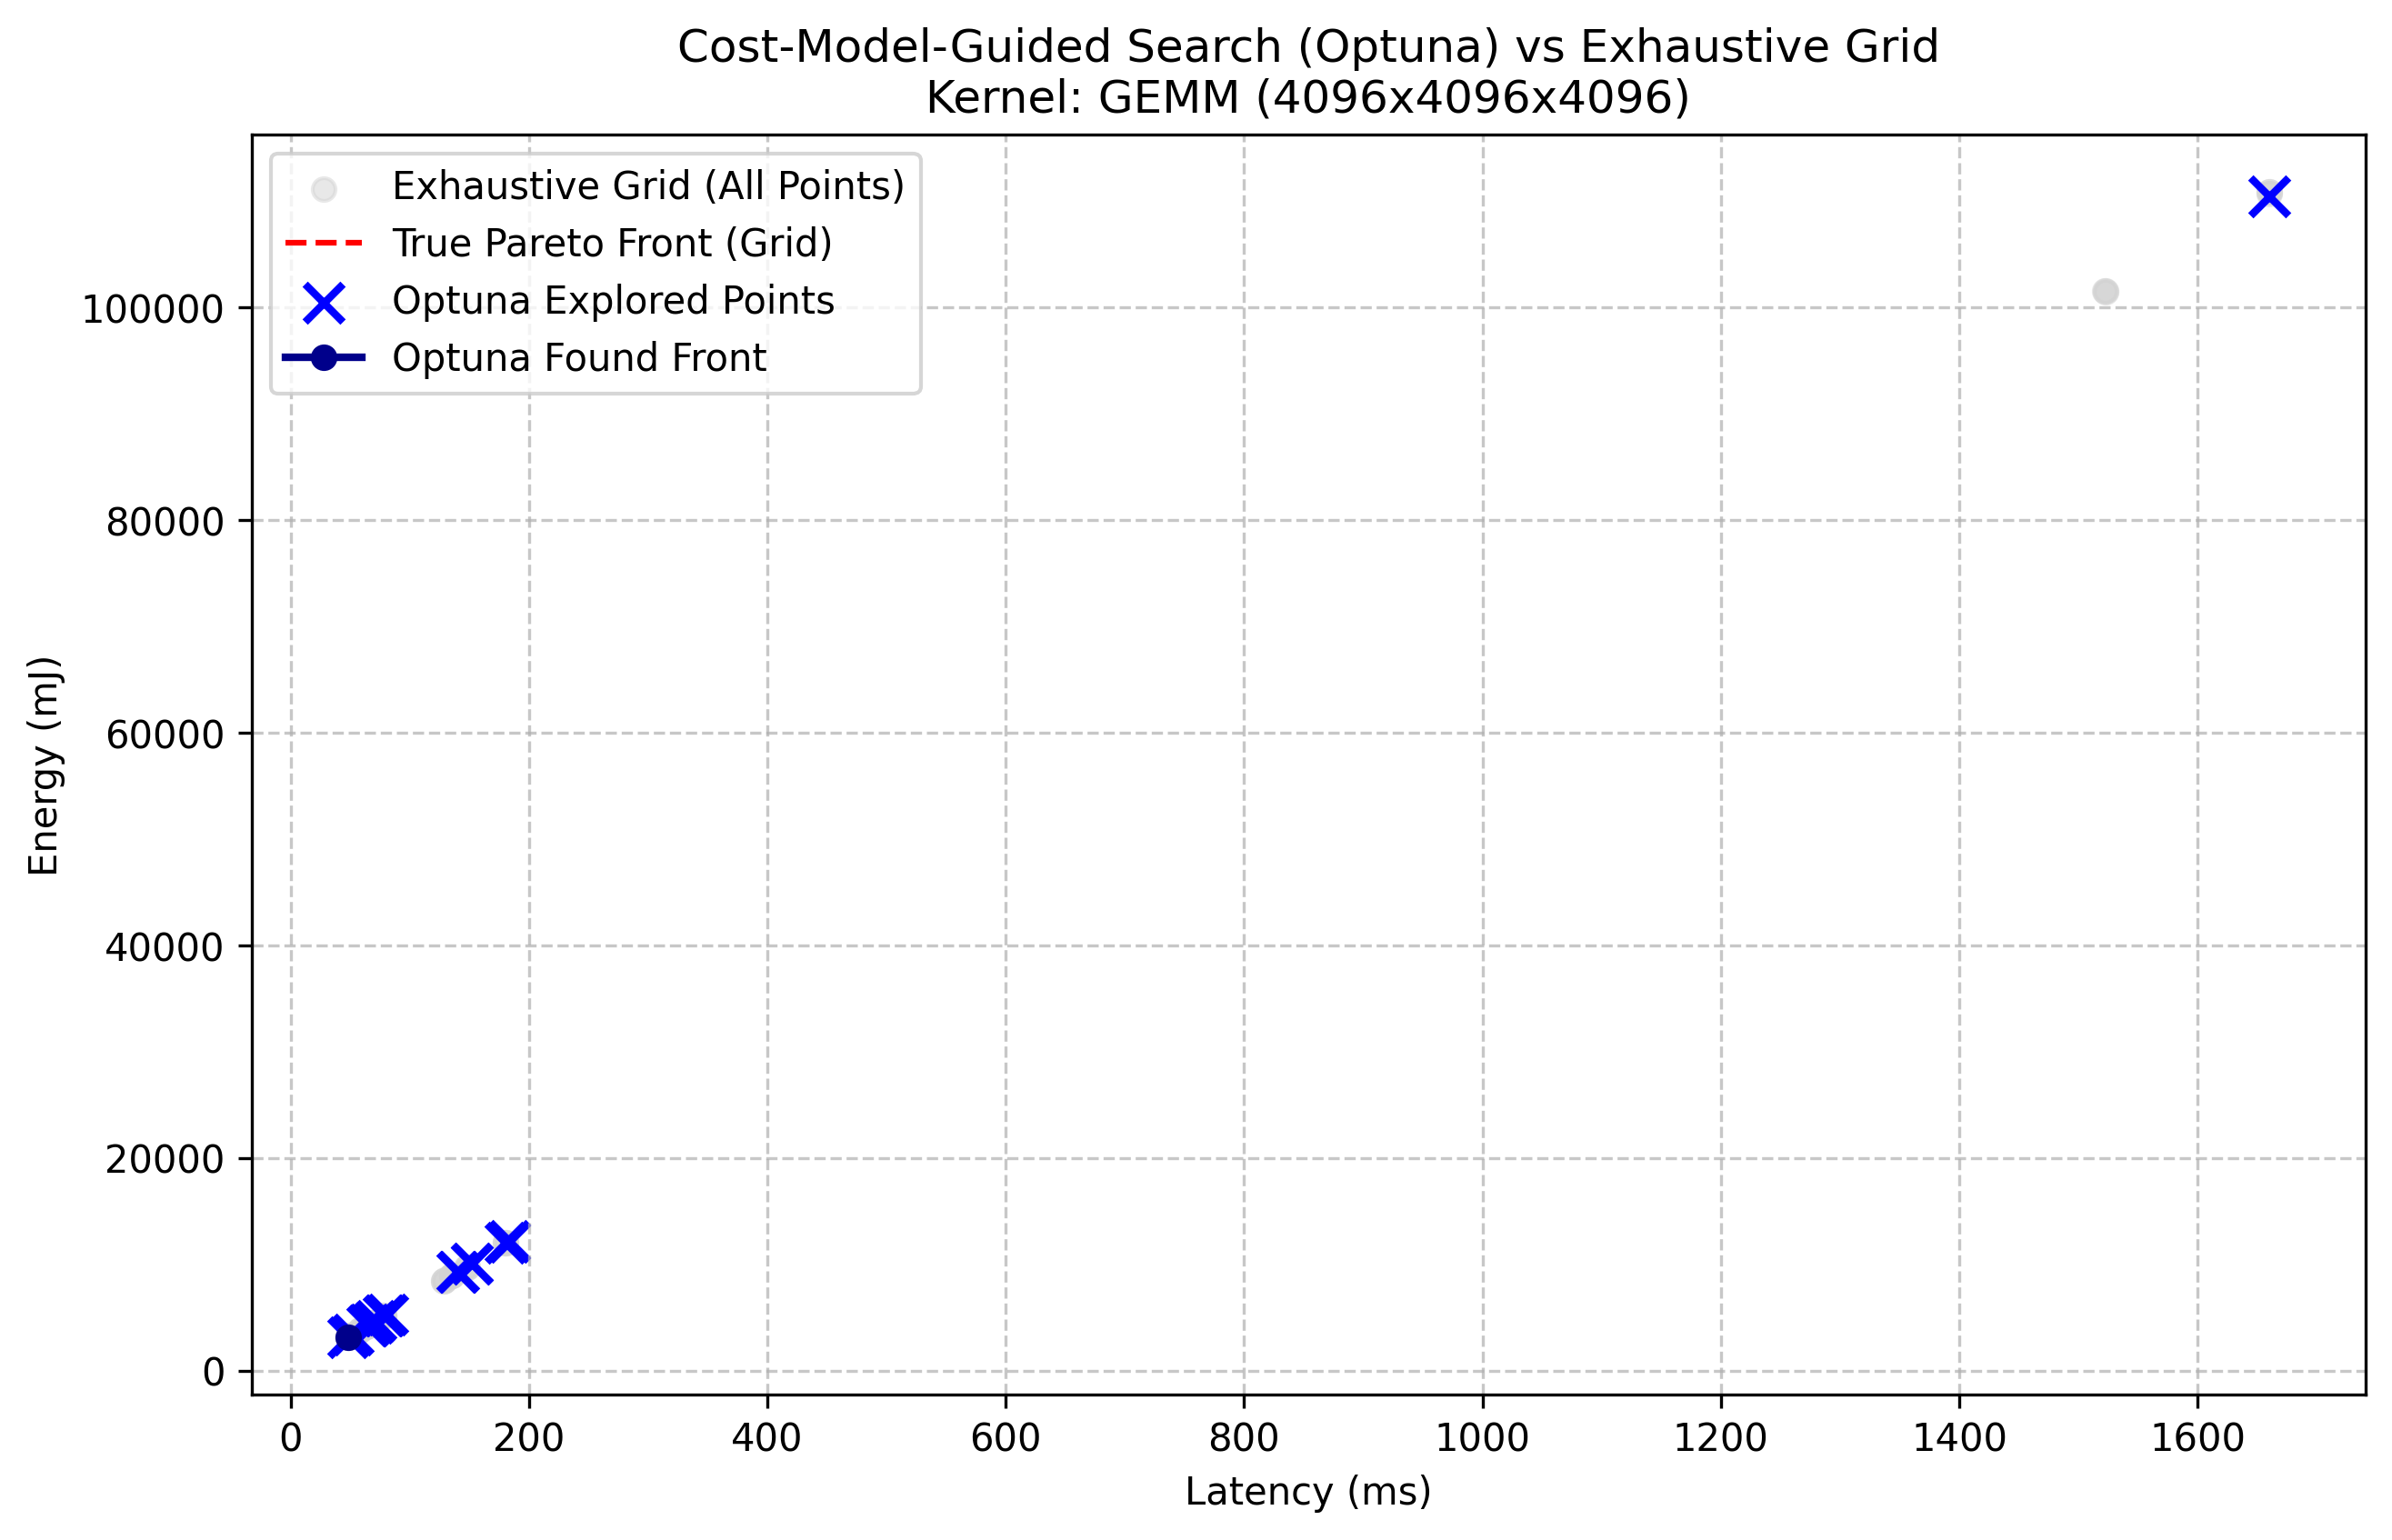
\includegraphics[width=\linewidth]{figures/optuna_vs_grid_pareto.png}
\caption{Optuna TPE Multi-Objective Search vs. Exhaustive Grid for Tiled GEMM ($4096^3$). Optuna successfully finds the Pareto knee within 20 trials.}
\label{fig:optuna_pareto}
\end{figure}
